
% This LaTeX was auto-generated from MATLAB code.
% To make changes, update the MATLAB code and republish this document.

\documentclass{article}
\usepackage{graphicx}
\usepackage{color}

\sloppy
\definecolor{lightgray}{gray}{0.5}
\setlength{\parindent}{0pt}

\begin{document}

    
    
\subsection*{Contents}

\begin{itemize}
\setlength{\itemsep}{-1ex}
   \item Questiomn 2: Hugget Model
   \item Quesion 3: Aiyagari
\end{itemize}
\begin{verbatim}
% Econ 527 Spring 2026
% HW 4
% Professor Greaney
% Written by: Camille Bergeron
% Due: May 22, 2026
\end{verbatim}


\subsection*{Questiomn 2: Hugget Model}

\begin{verbatim}
run('programs/PS4_huggett.m'); % run Hugget
\end{verbatim}

        \color{lightgray} \begin{verbatim}Transition probabilities:
    0.7351    0.2321    0.0305    0.0021    0.0001    0.0000    0.0000
    0.0387    0.7453    0.1945    0.0204    0.0011    0.0000    0.0000
    0.0020    0.0778    0.7514    0.1560    0.0123    0.0004    0.0000
    0.0001    0.0061    0.1170    0.7535    0.1170    0.0061    0.0001
    0.0000    0.0004    0.0123    0.1560    0.7514    0.0778    0.0020
    0.0000    0.0000    0.0011    0.0204    0.1945    0.7453    0.0387
    0.0000    0.0000    0.0001    0.0021    0.0305    0.2321    0.7351

File not found, calculating equilibrium interest rate distribution...
 
 Func-count     x          f(x)         Procedure
    1     -0.0150246   0.00325171        initial
    2     0.00659131      1.51304        golden
    3      -0.028384     0.187741        golden
    4     -0.0188175    0.0335984        parabolic
    5     -0.0103326    0.0162749        parabolic
    6     -0.0137713  0.000122134        parabolic
    7     -0.0135837  1.57918e-05        parabolic
    8     -0.0134659  2.48403e-07        parabolic
    9     -0.0134992  5.91309e-07        parabolic
   10     -0.0134326  3.12387e-06        parabolic
 
Optimization terminated:
 the current x satisfies the termination criteria using OPTIONS.TolX of 1.000000e-04 


Equilibrium r* = -0.013466
File not found, calculating hugget model...
Took 0.4351 seconds to converge
States at lower bound (a_min=-1.1103): 11
States at upper bound (a_max=55.5163): 0
File not found, calculating hugget net asset demands 
Took 12.6246 seconds to calculate
\end{verbatim} \color{black}
    
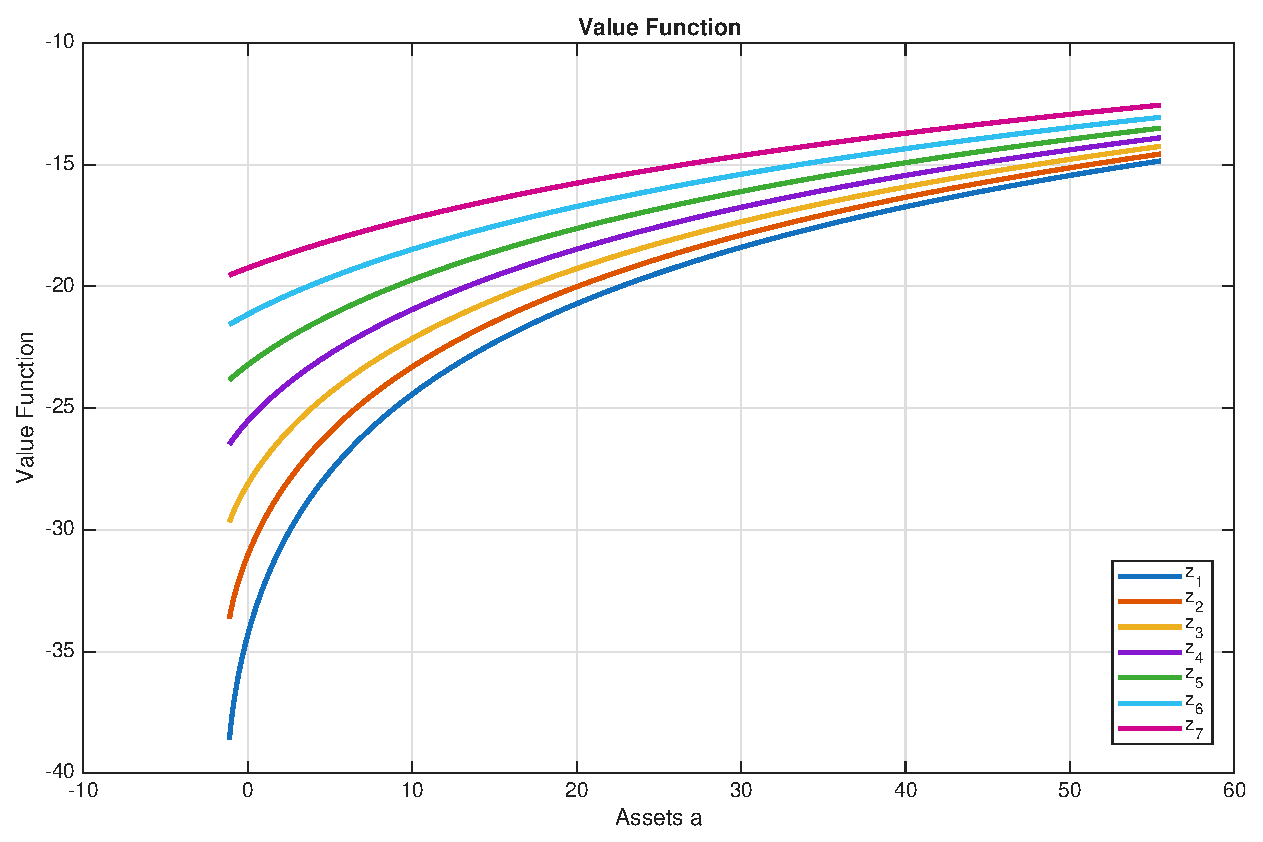
\includegraphics [width=4in]{PS4_run_01.eps}

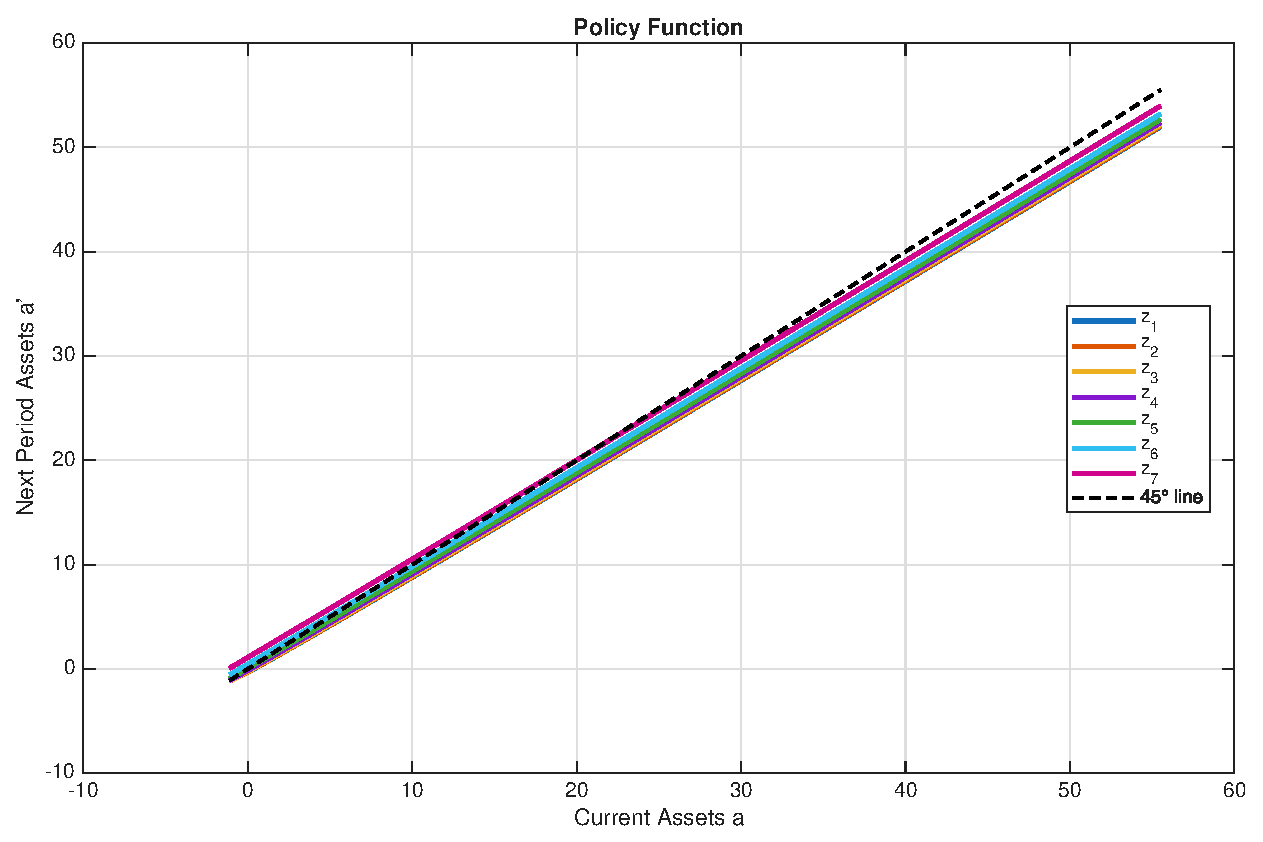
\includegraphics [width=4in]{PS4_run_02.eps}

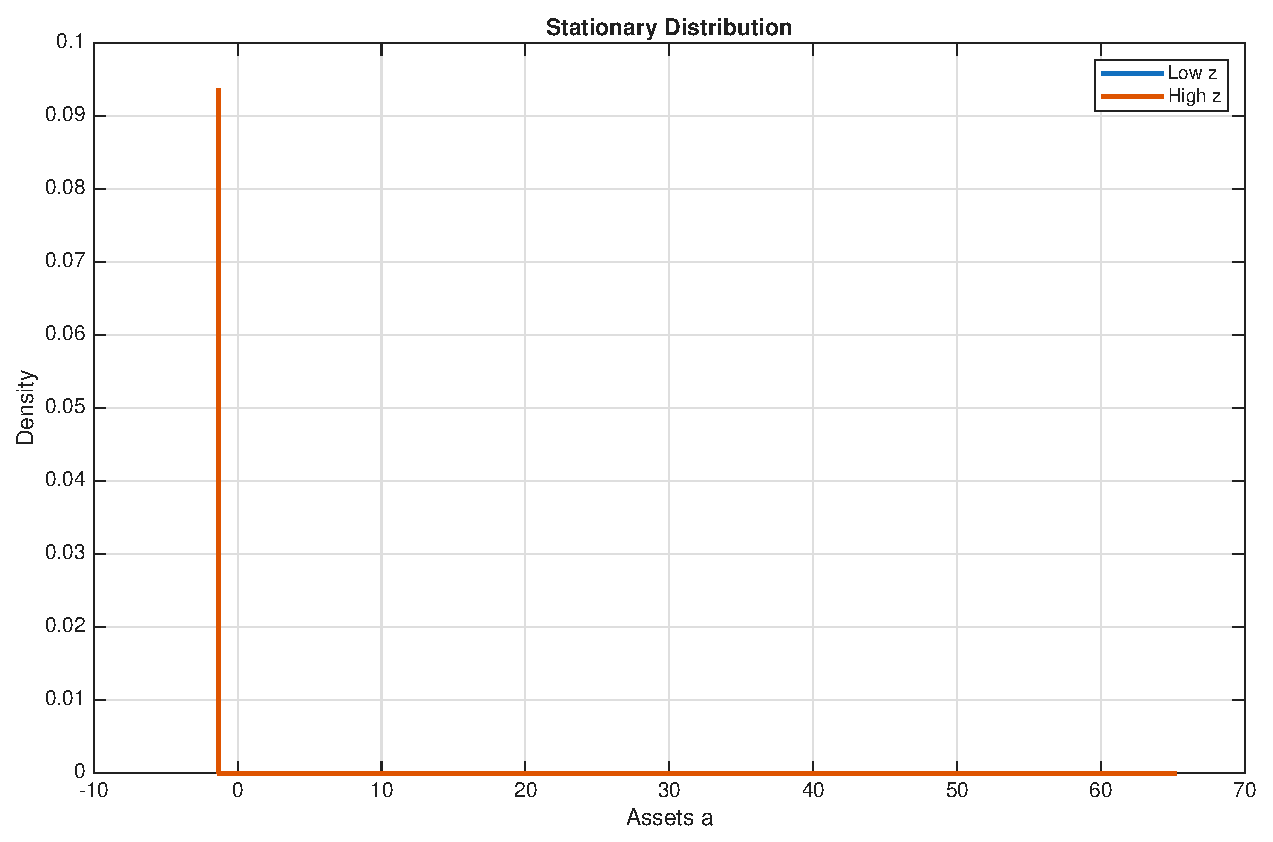
\includegraphics [width=4in]{PS4_run_03.eps}

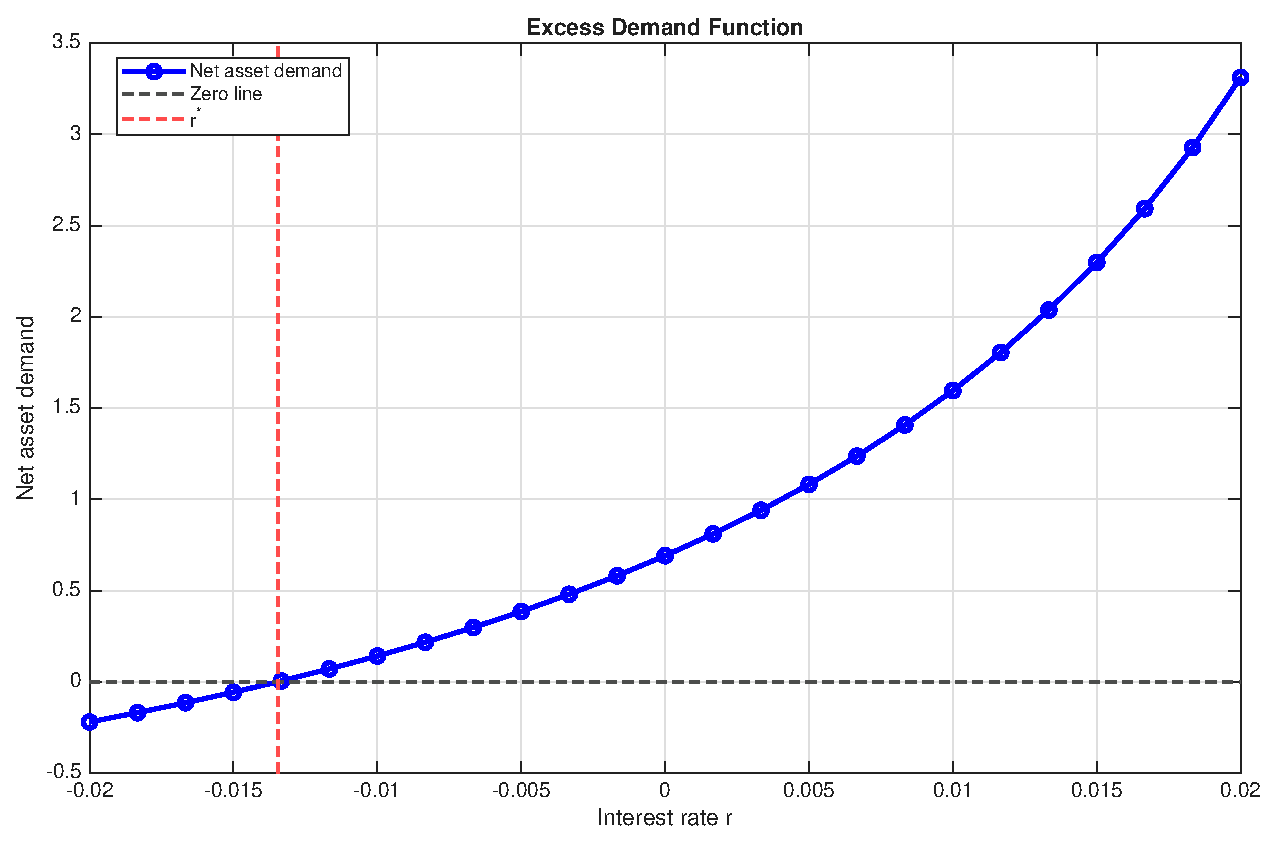
\includegraphics [width=4in]{PS4_run_04.eps}


\subsection*{Quesion 3: Aiyagari}

\begin{verbatim}
run('programs/PS4_aiyagari.m'); % run Aiyagari
\end{verbatim}

        \color{lightgray} \begin{verbatim}File not found — solving Aiyagari model...
iter    1 | k = 5.000000 | net_assets = 23.052835 | diff = 1.81e+01
iter    2 | k = 10.415851 | net_assets = 1.612913 | diff = 8.80e+00
iter    3 | k = 7.774969 | net_assets = 2.652661 | diff = 5.12e+00
iter    4 | k = 6.238277 | net_assets = 4.899017 | diff = 1.34e+00
iter    5 | k = 5.836499 | net_assets = 6.495597 | diff = 6.59e-01
iter    6 | k = 6.034228 | net_assets = 5.588198 | diff = 4.46e-01
iter    7 | k = 5.900419 | net_assets = 6.169092 | diff = 2.69e-01
iter    8 | k = 5.981021 | net_assets = 5.804459 | diff = 1.77e-01
iter    9 | k = 5.928052 | net_assets = 6.038617 | diff = 1.11e-01
iter   10 | k = 5.961222 | net_assets = 5.889653 | diff = 7.16e-02
iter   11 | k = 5.939751 | net_assets = 5.985155 | diff = 4.54e-02
iter   12 | k = 5.953372 | net_assets = 5.924184 | diff = 2.92e-02
iter   13 | k = 5.944616 | net_assets = 5.963225 | diff = 1.86e-02
iter   14 | k = 5.950199 | net_assets = 5.938271 | diff = 1.19e-02
iter   15 | k = 5.946620 | net_assets = 5.954240 | diff = 7.62e-03
iter   16 | k = 5.948906 | net_assets = 5.944028 | diff = 4.88e-03
iter   17 | k = 5.947443 | net_assets = 5.950561 | diff = 3.12e-03
iter   18 | k = 5.948378 | net_assets = 5.946383 | diff = 2.00e-03
iter   19 | k = 5.947780 | net_assets = 5.949056 | diff = 1.28e-03
iter   20 | k = 5.948162 | net_assets = 5.947346 | diff = 8.16e-04
iter   21 | k = 5.947917 | net_assets = 5.948440 | diff = 5.22e-04
iter   22 | k = 5.948074 | net_assets = 5.947740 | diff = 3.34e-04
iter   23 | k = 5.947974 | net_assets = 5.948188 | diff = 2.14e-04
iter   24 | k = 5.948038 | net_assets = 5.947901 | diff = 1.37e-04
iter   25 | k = 5.947997 | net_assets = 5.948084 | diff = 8.74e-05
iter   26 | k = 5.948023 | net_assets = 5.947967 | diff = 5.59e-05
iter   27 | k = 5.948006 | net_assets = 5.948042 | diff = 3.58e-05
iter   28 | k = 5.948017 | net_assets = 5.947994 | diff = 2.29e-05
iter   29 | k = 5.948010 | net_assets = 5.948025 | diff = 1.46e-05
iter   30 | k = 5.948015 | net_assets = 5.948005 | diff = 9.36e-06

Converged in 30 iterations (21.54 seconds)
r* = 0.022968,  w* = 1.171094,  K* = 5.948005

── Wealth Inequality ─────────────────────
Gini coefficient : 0.5381
Top 10% share   : 0.3421 (34.2%)
Top  1% share   : 0.0553 (5.5%)

States at lower bound (a_min = 0.00): 8
States at upper bound (a_max = 60.00): 3
File not found, calculating aiyagari net asset demands...
Took 16.5857 seconds to calculate
Warning: Ignoring extra legend entries. 
Warning: Exported image displays axes toolbar. To remove axes toolbar from
image, export again. 
\end{verbatim} \color{black}
    
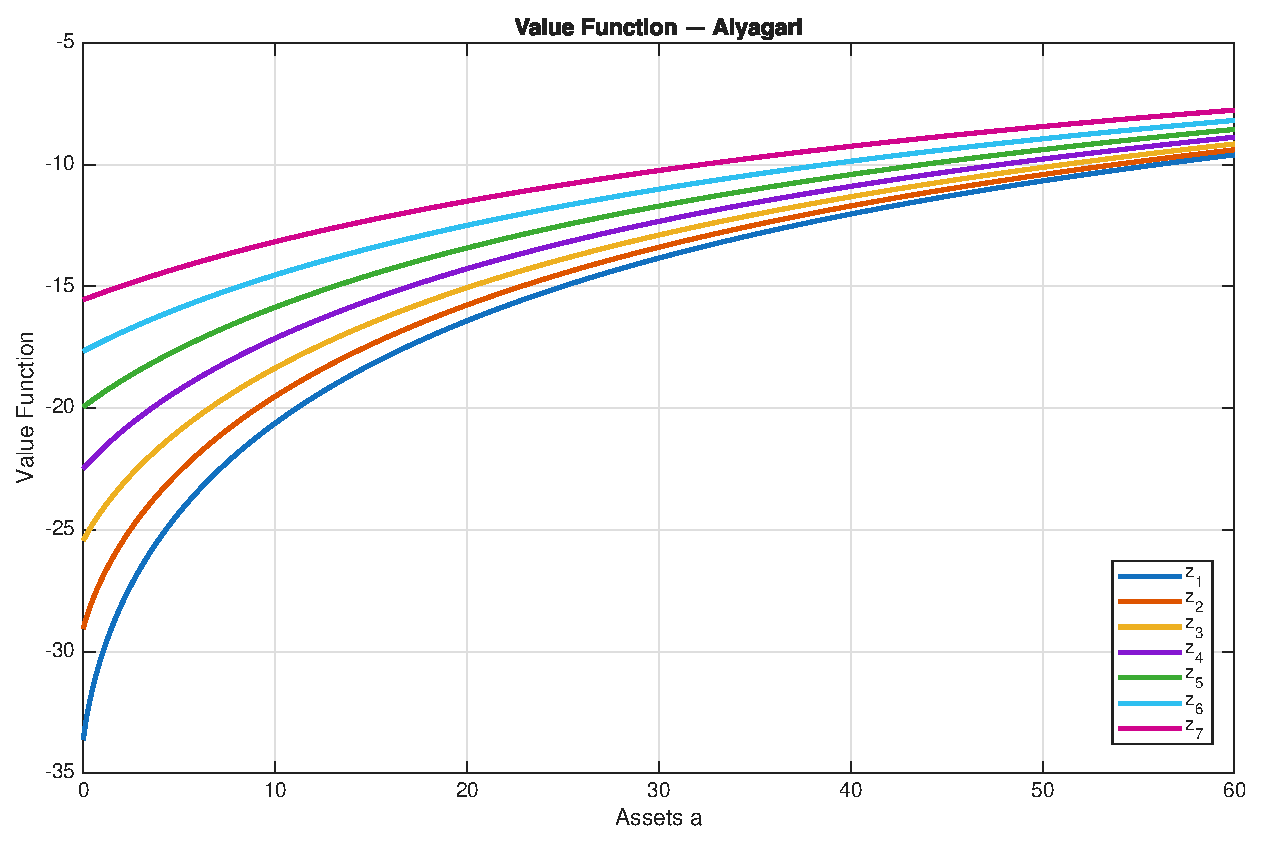
\includegraphics [width=4in]{PS4_run_05.eps}

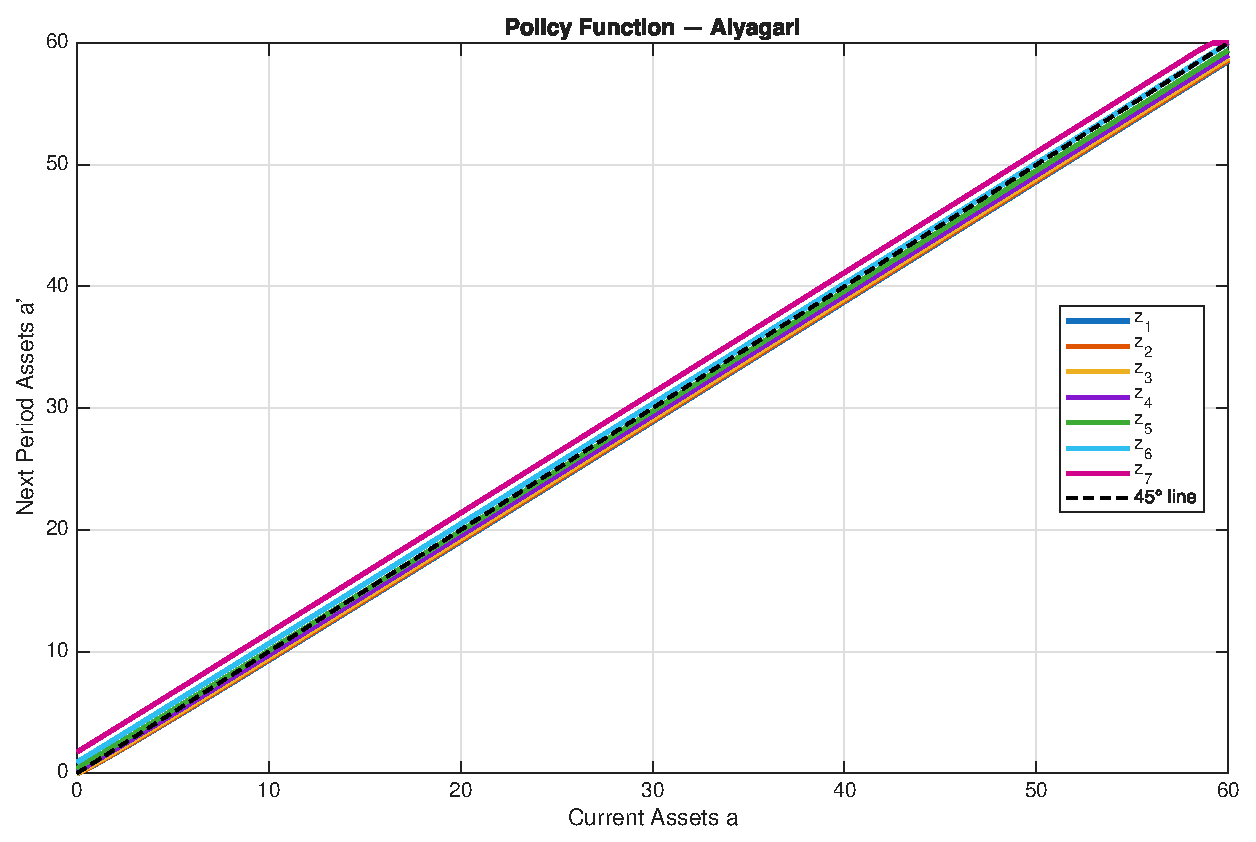
\includegraphics [width=4in]{PS4_run_06.eps}

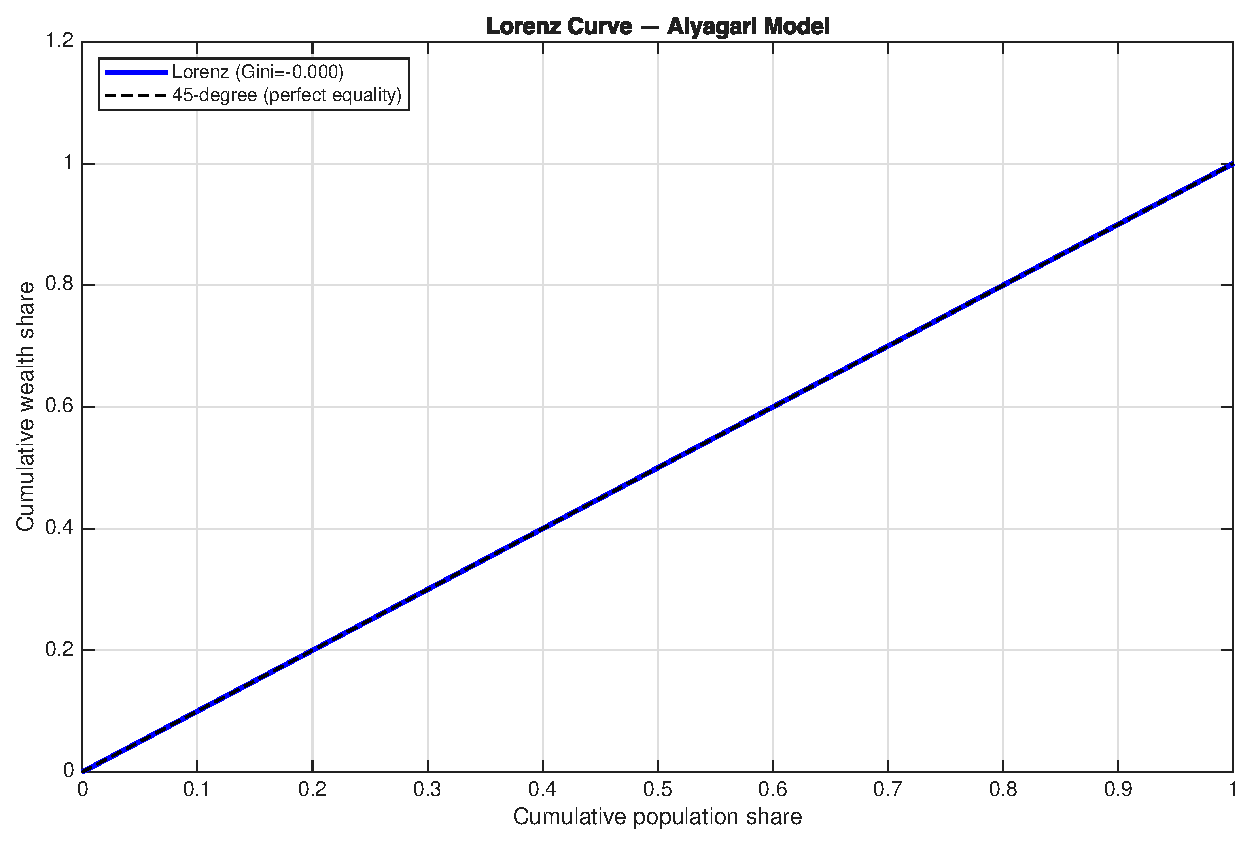
\includegraphics [width=4in]{PS4_run_07.eps}

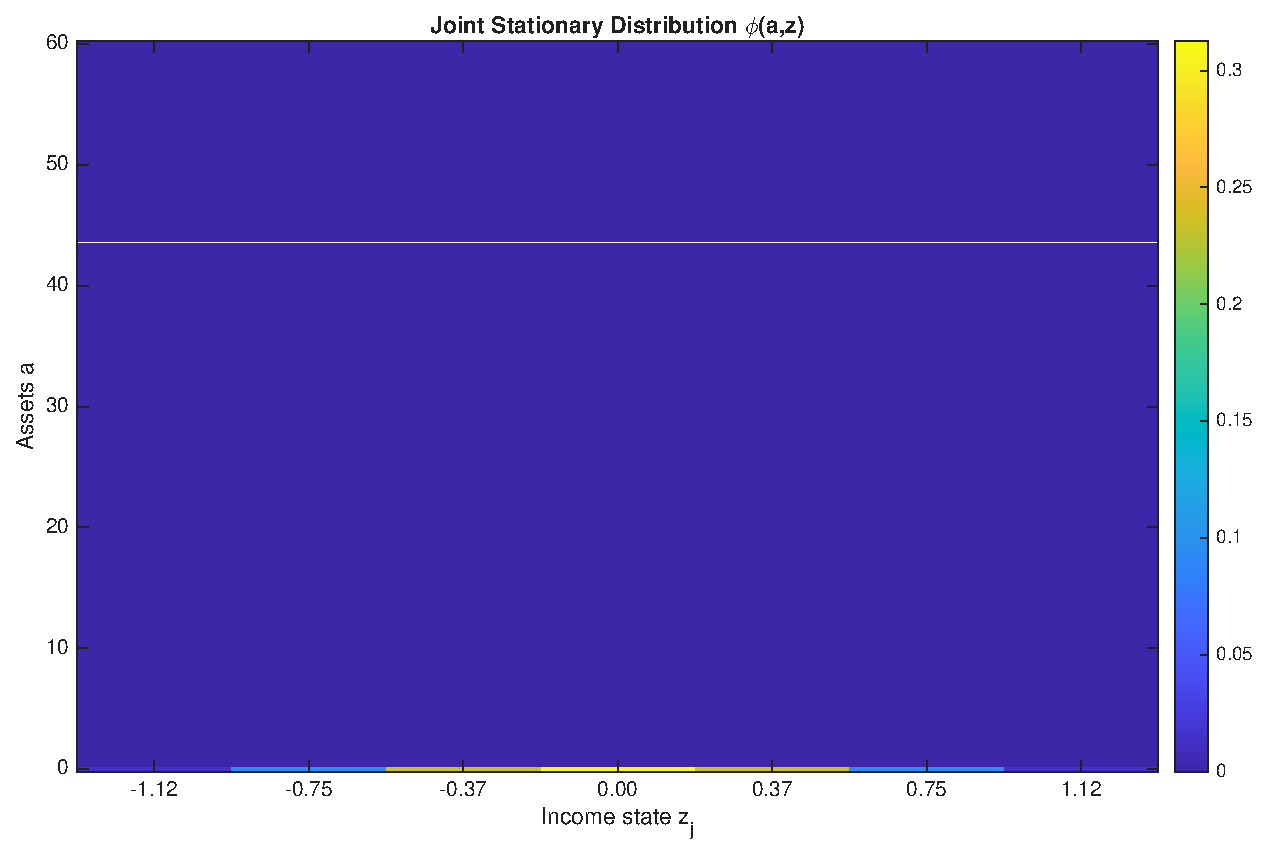
\includegraphics [width=4in]{PS4_run_08.eps}

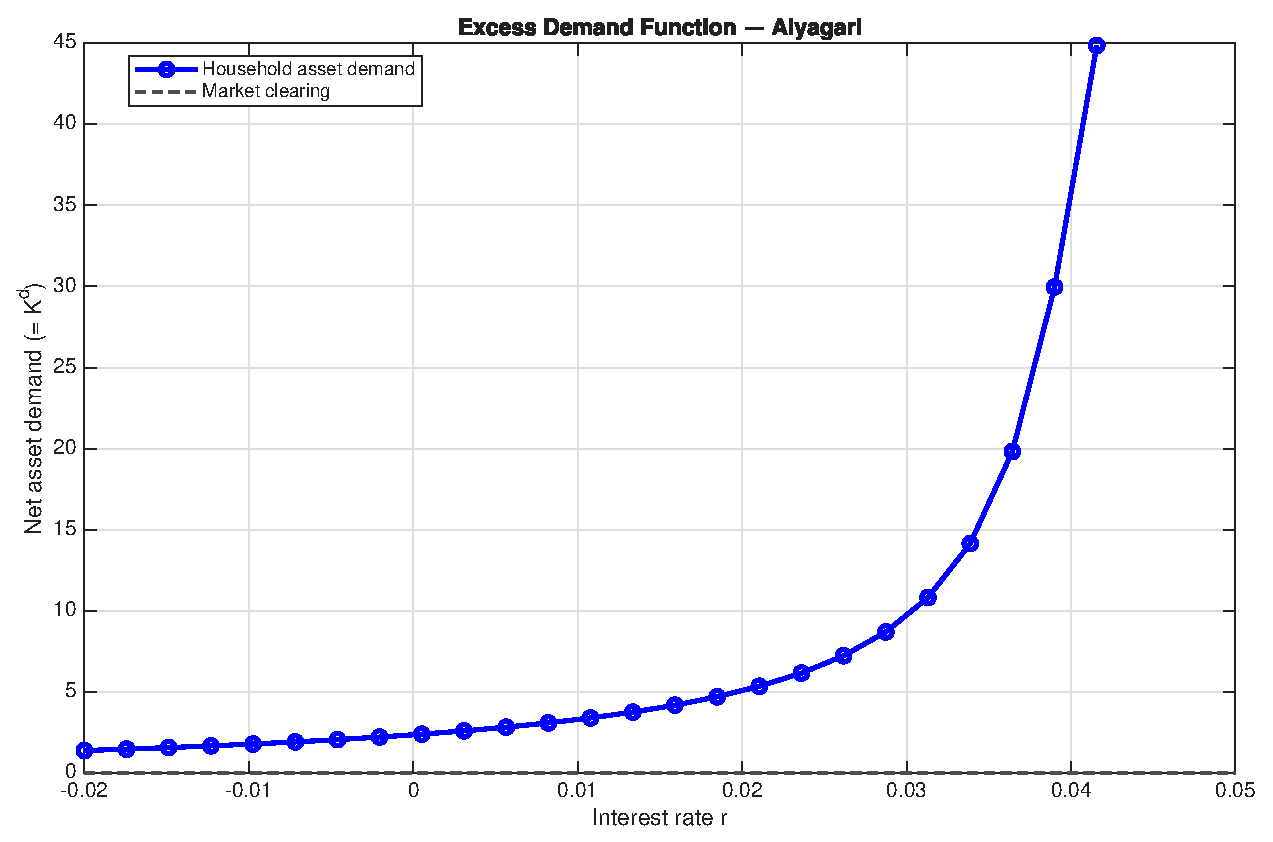
\includegraphics [width=4in]{PS4_run_09.eps}



\end{document}

